%%%%%%%%%%%%%%%%%%%%%%%%%%%%%%%%%%%%%%%%%%%%%%%
%\chapter{Scaffolding Citizen-led Complex Knowledge Work}
\chapter{Social Computing for Complex Work}


\begin{quote}
\emph{Social computing platforms enable people to connect and share but provide little to no support for deeper work}. This dissertation provides a novel approach for complex work by introducing procedural guidance in social computing. Systems instantiating this approach integrate theories from learning, collaboration, and interface design. Supporting people in personally meaningful activities such as generating and evaluating scientific theories provides multiple advantages: people can answer their own questions, the world can learn something new, and our future society can potentially have more diverse stakeholders and contributors.
\end{quote}
\vspace{0.25in}

Social computing platforms have revolutionized how people connect, communicate, and share. Friends and family stay in constant touch about both significant and mundane life events. Strangers from around the world discuss ideas about topics of mutual interest. Increasingly, these opportunities to connect and share have also translated to more active doing: people fund ideas that traditional business places might balk at~\cite{hui2014understanding}. Others have used social platforms to bring attention to important political, and economic questions~\cite{tufekci2012social, fox2017social}. By altering how we communicate and chat, social platforms have cemented a central place in our professional, personal, and leisure activities. However, the benefits of social computing are not distributed equally. 
%for instance, people in Sudan have taken down dictators [??]. 

%xx\% of the most popular posts on Twitter are from experts
Every internet user has a voice but some amplify them better than others: people's online informaking seeking behavior is a significant predictor of their existing social capital~\cite{gil2012social}. Widely accessible research papers and articles provide useful learning materials; however, evidence-based rational discourse on online fora are an exception, not the norm. Social computing platforms have vastly succeeded at keeping people engaged with careful interface design but they barely support \textit {citizen-led enquiry}. These examples suggest that simply connecting people is not enough for successful citizen-led work. Absent tools to build expertise, social computing seems less of a transformative panacea. How might people succeed at their goals using online systems?
%While anyone can create an online group on a topic of interest, most online communities fail to sustain this interest beyond a few weeks [??]. 
%When people discuss people create faulty insights from self-tracking and conspiracy theories abound.
% 1 to 1 link with the first para

%%interactive vis (social computing discussions) is awesome
% people can do stuff with hypotheses (test them?)
%    however, viz is hard (scientific work)
%        programming toolkits needed and impose burden (support needed to get started, reduce burden, and …)

%\subsection{Pivot to people - People can do great things but need help...}
%Well, what are people good at? What are they motivated to do? 

%People have complementary knowledge in comparison to experts and are uninfected by expert biases; these insights are drawn from lived experience, both individual and collective.
%Specific to this dissertation: 
People have strong personal motivations and contextual insights; they possess a remarkable ability to identify patterns and create theories from their lived experiences~\cite{Gelman2011}. While people have an amazing breadth and depth of ideas, they lack the expertise to implement these ideas. To create knowledge, they need mental scaffolds for organizing complex work, domain knowledge to compose and execute the steps, and ways to ask for help. Experts benefit from conceptual knowledge, professional training, pre-existing organizational structure for collaboration, and direct access to resources. Currently, citizens lack these resources. By performing personally meaningful work, people can answer their own questions and their ideas can catalyze creating new knowledge. As a result, both individuals and the world at large have missed out on this this opportunity for useful work. How might online systems support citizen-led knowledge work? 

%this is the current state --  this is the big challenge, why is it a challenge
%% however, scaling good teaching is hard - kulkarni
%     this peer thing can be helpful (evidence from small studies)
%        however, this is challenging — 2 causes
%        interfaces need to provide scaffolding 


%Let''s reflect on this dual nature:  science can answer life-relevant questions but few know how to even get started. As a result, people fail to answer their questions and institutional science misses out on ideas from beyond the ivory tower. 

%one line to summarize my work -- see other intro
%two properties of classes help us - kulkarni
%this thesis leverages these two properties and provides a new class of benefits etc... 
%what helps us
%1. the scientific method is structured
%    1. even though creative and open-ended
%2. roles: people take them online
%    1. captures diversity — breadth
%    2. micro-expertise supports this explicitly 
%3. procedural learning: can teach people how to do things
%    1. captures learning — depth

This dissertation advances the design of social computing systems by integrating learning and collaboration for complex work such as generating and evaluating scientific theories. Over 600 people from 30 countries have self-organized to generate theories about the human microbiome and test them by running experiments. Gut Instinct emodies this insight and introduces a collaborative citizen science platform for people to transform lived experience into scientific theories. This dissertation raises the question: how can global communities create knowledge that meets their goals without waiting for experts to lead?

\begin{figure}[b] 
  \centering
  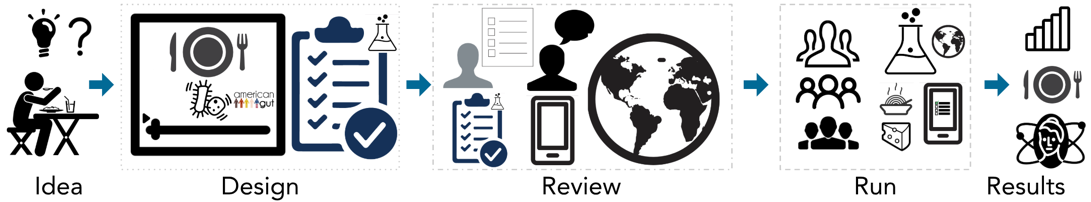
\includegraphics[width=1.0\textwidth]{figures/intro/intro-1}
  \caption[The Gut Instinct platform enables anyone to transform their intuitions to hypotheses 
and then design and run experiments to test them]
{The Gut Instinct platform enables anyone to transform their intuitions to hypotheses 
and then design and run experiments to test them~\cite{Pandey, Pandey2017,Pandey2018}. Gut Instinct integrates 
conceptual learning embedded via short lectures and software-guided procedural 
learning to enable designing and reviewing experiments. Participants from around
 the world join experiments, follow instructions, and provide data in response to 
automated data collection reminders. }
  \label{fig:intro-1}
\end{figure}

%%%%%%%%%%%%%%%%%%%%%%%%%%%%%%
\section {Current online designs do not support deeper work}
People’s curiosity and needs provide endless possibilities to perform useful work. People design, build, and track to better understand and improve their health~\cite{DanaLewis}. However, traditional social computing designs don’t funnel this motivation to useful work. 

On numerous online fora, people share their intuitions, observations, folk theories, and even results from trying different approaches to improve their health, e.g. from simple ideas like ‘giving up drinking coffee to improve quality of sleep’ to testing different dietary approaches. 
%However, online fora encourage long, rambling discussions that makes it difficult to identify signal from noise. 
Current online forum designs prioritize discussion---sharing personal details in long, free-flowing text---over goal-directed structure and learning~\cite{Thomas2002}. While learning resources like Massive Open Online Courses (MOOCs) abound, they adopt traditional classroom pedagogy through lectures focused on conceptual knowledge. Synthesizing the social computing literature highlights three challenges: poor signal-to-noise from crowds due to lack of training~\cite{Doroudi2016a}; inefficient collaboration without careful attention~\cite{Resnick2011}; and poor results (or no results at all) unless experts lead. Desirable social computing techniques will reliably enable a wide variety of people to contribute more than they naturally could and manage the dependencies among a large set of tasks. 

%To summarize, lack of appropriate ``learning abstractions'' make complex work unrealistic.

%Two major issues in enabling complex work on the internet are improving quality of individual contribution and 
%managing overall contributions to make complementary. 
%(diversity and scale?) 

%To address these concerns, this dissertation introduces and evaluates 
%peer production architectures and procedural learning.

%Some draw ideas from current research by reading and discussing papers. In some cases, these discussions are not just anecdotal but also derive from state-of-the-art scientific work. In some cases, people contribute back to scientific work as well. 
%How can social computing platforms effectively enable people to do more personally meaningful work built upon their experiences and insights?
%The goal is to create environments for learning and collaboration through complex, personally meaningful work.

%%%%%%%%%%%%%%%%%%%%%%%%%%%%%%%%%%%%%%%%%%%%%%%%%%%
\subsection{Challenge: Designing support for collaboration and knowledge requirements}
While people are connected online and collectively have access to many resources, they need ways to collaborate effectively. 
In a large distributed community, there’s often someone who happens to 
have important relevant knowledge, usually drawing on a relevant but 
distant domain. Such distributed efforts are a type of lead-user innovation~\cite{VonHippel2005a}. 
Having many people work on the same problem increases the odds that 
one will break through. Drawing on secondary expertise as inspiration can
 be an important agent of creativity because almost by definition, the 
combination is rare~\cite{Boden2004}. While many hands make light work, novices need clear contribution opportunities. 

%People lack the expertise to know what to do and how to do it. 
Citizens have a different background than professional scientists; they have unique
 personal experiences but lack the years of domain training. Novices are also
\textit{uninfected} by all the knowledge that enables experts to
innovate. Success with complex creative activities requires procedural
knowledge (how to do things) in addition to conceptual
knowledge (facts). While many resources offer facts, procedural
learning is often ignored. 
% kulkarni -- "This assessment requires bothcommon-sense knowledge to understand student work and the expertise to assess tacit criteria such as “well-designed” or “well-modularized” that cannot be completely articulated. Indeed, teaching such tacit criteria is an important goal in open-ended domains like design"


%The crowdsourcing literature offers many good verification approaches for tasks 
%with clear right or wrong answers – like whether two images represent the same 
%product or what street number is written on a sign. However, verifying knowledge
 %work necessitates a different approach because it requires making 
%situationally-appropriate choices. 
%Furthermore,  how do people ask others for help? Who do they reach out to?

%Open \& crowd innovation builds up on contributions
%by diverse online participants, and a ‘bubbling up’ process for strong ideas~\cite{Yu2012}.

To summarize, supporting complex work with social computing requires two key features: 
1) careful collaboration primitives, and 2) procedural support for deeper individual contributions.


%todo-introduce the learning and collaboraiton taxonomy here
\begin{figure}[!h] 
  \centering
 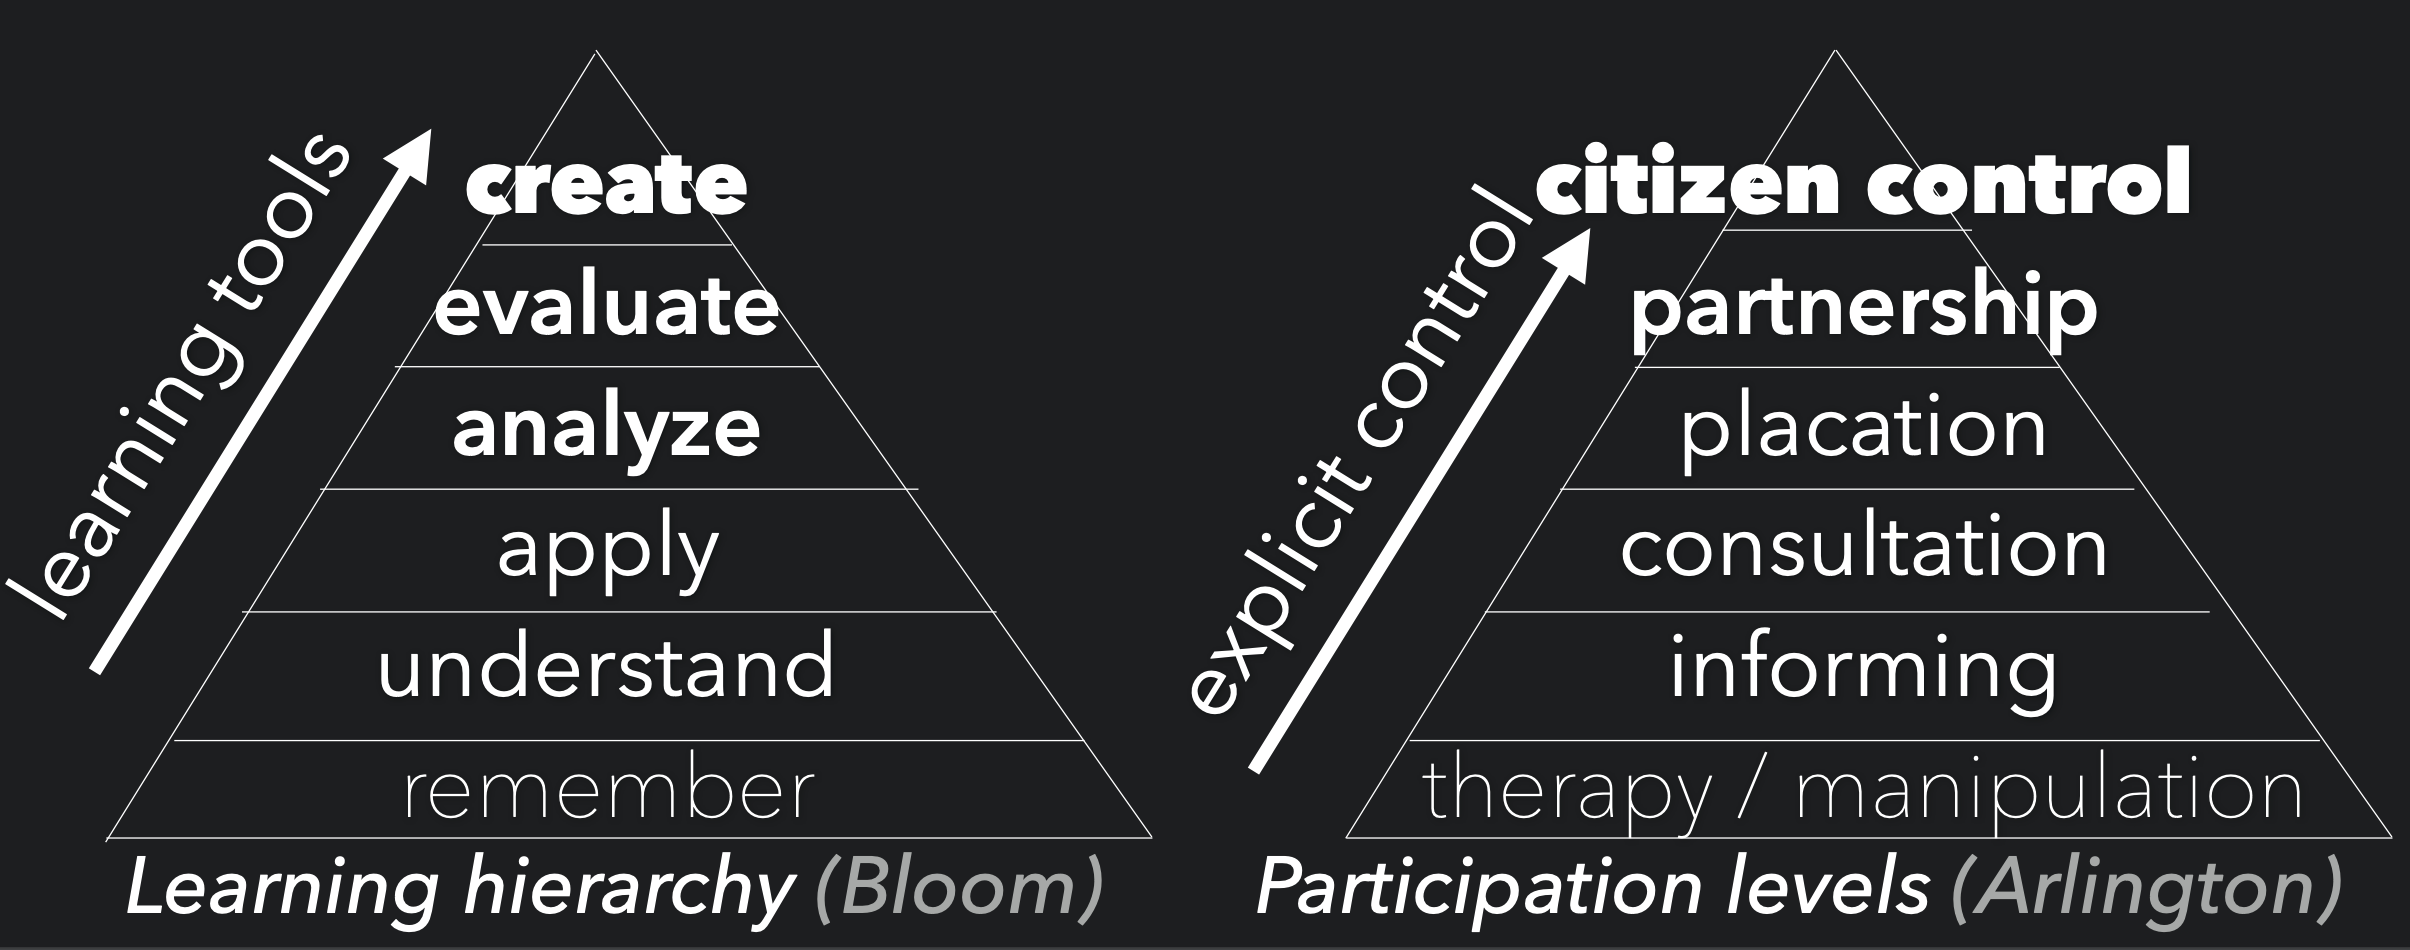
\includegraphics[width=1.0\textwidth]{figures/intro/intro-taxonomy}
  \caption[Drawing from Maslow's hierarchy of learning and  hierarchy of contribution]
{Drawing from Maslow's hierarchy of learning and Arlington's hierarchy of contribution}
  \label{fig:intro-taxonomy}
\end{figure}

\subsection{Scientific experimentation: An instance of complex knowledge work}
%here''s an example: experimentation 
Many people are interested in understanding and improving their health. Millions of peple from all over the world share their insights. 
Why haven't people run experiments to test these ideas? Scientific experimentation features technical requirements and contextual choices 
that are inscrutable for a lay individual yet necessary for success~\cite{Martin2007}. While 
professional scientists and commercial ventures run experiments every day, with 
notable exceptions~\cite{Cooper2010,DanaLewis}, empirical papers from non-professionals are 
vanishingly rare. This biases the questions asked, studies run, and knowledge 
created~\cite{Henrich2010a}. People have questions about their health, but lack the expertise 
and resources to scientifically investigate them. Broadening the pool of 
experimenters could help people investigate their curiosities, develop solutions 
to improve health and performance, and assist institutional researchers. To create computational systems that leverage people's strengths and mitigate the lack of training, this dissertation focuses on scientific domains that are nascent, highly contextual, and personally motivating.

%%%%%%%%%%%%%%%%%%%%%%%%%%%%%%%%%%%%%%%%%%%%%%%
\section{Thesis Statement and Contributions}
This dissertation investigates the question: how might online platforms enable people perform 
complex work that is personally meaningful work? Underlying these investigations is the thesis:\\
%"My thesis statement is"
\begin{quote}
\emph{Procedural guidance in social computing catalyzes personally meaningful \& useful scientific work}
\end{quote}

This dissertation\textquotesingle s primary contribution is the idea of intergrating learning in social computing tfor groups of novices to perform complex, creative activities. The thesis achieves this integration by building a sequence of interactive prototypes that enable people to collaboratively generate and test hypotheses. In the process, the prototypes divide complex work into distinct activities: self-sourcing the design and crowdsourcing people's inputs and data. Every prototype advances social computing further as a domain for deep, personally meaningful work. Beyond introducing learning abstractions, this dissertation carefully designs the affordances in the system to enable different users for different needs. 

 %To realize this idea, 
This dissertation makes three types of contributions: theoretical perspectives / techniques, real-world systems, and outcomes including empirical results.
%including empirical results, systems lessons, and datasets. 
%(Figure \ref{fig:contributions}). 
%todo - make and add this

%%%%%%%%%
\subsection{Theoretical  Techniques}
Improving  work quality in social computing suggests deepening individual contributions and broadening participation by providing different contribution mechanisms. The former requires better learning tools and the latter requires better collaboration tools and dependency management. Consequently, this thesis' theoretical contributions include 1) principles to integrate guidance for complex tasks, and 2) ways to divide complex tasks into multiple roles or affordances.

%“..adapts and extends techniques from xxx” -  arvind
%system-led learning vs people-led
%Traditional systems think of knowledge as being provided by the people, while we being the knowledge from the system itself.

% come up with principles myself
%figure about conceptual and procedural learning 
\textbf{Principles to integrate learning in social computing}: Learning broadly comprises conceptual (declarative) and procedural knowledge. Conceptual learning---the primary focus of classroom teaching---involves understanding and interpreting concepts and the relations between concepts [Arslan 2010]. In contrast, procedural learning teaches "action sequences for solving problems" [Wagner99]. To contribute usefully, people need to have a good working model of both the concepts and procedures for an activity. This dissertation enables knowledge acquisition in two ways: 1) reifying conceptual bits in the software; and 2) providing procedural guidance with examples, checklists, and templates. These techniques aim to move individual contributions to higher levels on Maslow's hierarchy (Figure~\ref{fig:intro-taxonomy}). 
%todo-show how my system does that
Specifically, Docent's Learn-Train-Ask workflow (Chapter 4) embeds procedural guidance about hypotheses while Galileo's design workflow (Chapter 5) demonstrates the efficacy of reifying the genre of between-subjects experimentation in the software itself.
%https://teachingmathliteracy.weebly.com/conceptual-vs-procedural-knowledge.html
%rittle-johnson and wagner


\textbf{Ways to decompose a complex activity}: 
Individuals, groups, and machines possess complementary strengths. Individuals might be highly motivated on a topic of personal interest; their lived experiences provide ideas that might be potentially novel. Groups of people might be less motivated but provide another set of eyes and complementary knowhow and insights from lived experiences; their efforts can help check slips from the creator and provide novel inputs. Finally, computers can implement things consistently to reduce biases but they cannot interpret open-ended instructions fairly in different contexts the way people can. Given these complementary strengths and limitations, this dissertation suggests the following process: 1) support an individual in creating an initial design on a personally meaningful topic; 2) improve it with others' feedback to create an actionable plan; and 3) implement the plan with the help of automated software. For all these steps, the system manages the interdependencies beneath the sheets. Arlington proposed this thing -- TODO ---. This dissertation aims to push collaboration up Arlington's hierarchy (Figure~\ref{fig:intro-taxonomy}). 
% (todo- fix this to crisp english writing) (see slide deck)

%The efficacy of these techniques is borne out over multiple deployments. All these techniques have been put in systems as interfaces, intelligent backends, and so on... \\

%fig - present a stack of things

%\begin{figure}[t!] 
%  \centering
%    \includegraphics[width=1.0\textwidth]{figures/img/intro/1-contributions}
%  \caption[Contributions of this dissertation]
%{Contributions of this dissertation including empirical results theoretical perspectives/techniques, real-world systems, and multiple outcomes}
%  \label{fig:contributions}
%\end{figure}

\subsection{User Interface and System Design}
%User interfaces and system design for efficient implementation
%figs needed to explicate 

%todo-reconsider
%(introduce roles)
When trying to leverage guidance and roles for complex citizen work, two challenges emerge. First, the internet is a diverse community: people might have poor models of reasoning and frame their ideas and intuitions in weird ways. The software should be understandable to a broad range of participants. Second, complex activities are challenging: the interface should make it easy for people to focus on the current step and provide resources to get unstuck. Designing such a system requires walking a fine line: too much information might overwhelm people while too little make people struggle. These techniques need to be baked in simple, interactive interfaces.
%; therefore so we need UIs for focused collaboration. 

%System contributions
To demonstrate the efficacy of these ideas, this dissertation introduces Gut Instinct, a collaborative citizen science platform for people to transform lived experiences into scientific theories. Gut Instinct frames the task of hypothesis-testing as a crowdsourcing problem, develops techniques and platform that supports different roles with just-in-time learning, and provides efficient backend support to automate simple tasks. Gut Instinct divides multi-party collaboration into complementary tasks and supports them using different contribution mechanisms (like adding a question, editing a response) and roles (like experimenter, reviewer, participant). This provides people the flexibility to choose how much they’d like to contribute. Finally, Gut Instinct automatically manages multiple activities to reduce 
bias and experimenter/participant workload, such as randomized placement of  people into conditions, maintaining anonymity, and collecting and cleaning data.

%%"Furthermore, adding location information to photo collections is by itself insufficient for scenevisualization: we also need intuitive, interactive interfaces for exploring these scenes. There are several challenges faced in the design of such interfaces. First, unlike with Google Street View, where photos are taken at regular intervals, personal or Internet collections are typically an unstructured soup of photos. Nevertheless, the navigation controls should still be intuitive and exhibit regularity. Second, such controls should make it easy to find and explore the interesting parts of a scene, particularly for tourist sites."

%%%%%%%%%%%%%
\subsection{Outcomes}
%\subsubsection{Empirical Results from Real-world Deployment}
%expertise: limited; diversity: different countries; scale: some

%\subsubsection{Dataset}
%1. repo of hypotheses with rating
%2. repo of experimental designs
%3. ...

%\subsubsection{Impact}
This dissertation demonstrates how we might draw on people’s diverse background knowledge, interest, and micro-expertise to expand scientific knowledge and push it in new directions. More specifically, the Gut Instinct platform instantiates these ideas enabling participants of the American Gut Project (the world’s largest crowdfunded citizen science project) to generate and experimentally investigate hypotheses. 344 volunteers from 27 countries created 399 hypotheses about their health and the gut microbiome. Remarkably, microbiome scientists rated a fifth (75) of these hypotheses to have a scientifically valuable insight about a topic not covered by existing published work. Volunteers fleshed out 60 of these hypotheses into complete experimental designs. My entire work (code + data) is open source so others can edit, build, and experiment.

This dissertation has also enjoyed sufficient support in multiple research communities: Innovation researchers at MIT, online and offline fermentation and self-tracking communities, and citizen science groups. Finally, parts of the system have been taught in classrooms including CSCI 499: (Computing for Social Good) at USC. 

This work explores how online learning and process training systems, combined with
peer collaboration, can help people learn similar skills that
can be useful in scientific and design domains.


%%%%%%%%%%%%%%%%%%%%%%%%%%%%%%%%%%%%%%%%%%%
%\section{Dissertation Roadmap}

%%%%%%%%%%%%%%%%%%%%%%%%%%%%%%%%%%%%%%%%%%%%%%%%%%%%%%%%%%%%%%%%%%
%todo- “we” refers to the set of authors…  -- see arvind



%This dissertation creates the opportunity of harnessing humanity\textquotesingle s collective efforts to accomplish great goals.

%"double quotes"


%The techniques make the idea concrete; the system operationalizes the techniques and makes them work; and the outcomes discuss the successes and failures of our approach.

%to people for them to perform personally meaningful work.
%My research prototypes collective systems for large-scale problems.
%Worldwide, people use online health fora to share insights and look for answers
%Iin short, to push people towards actively testing their ideas rather than just sharing them?  whether drinking kombucha really changes the gut constitution? In the absence of support and guidance, how can people do more? . 

%%1. novice-led
%    1. no experts
%    2. with other novices 
%2. personally meaningful 
%3. techniques
%    1. expert work to social computing 
%        1. ways to do that
%4. output
%    1. create new knowledge 
